% \usepackage{graphicx}
\renewcommand{\arraystretch}{1.2}

\noindent
% \resizebox{\textwidth}{!}{%
\begin{tabularx}{\textwidth}{!{\vrule width 1pt}>{\songti\centering\arraybackslash}m{4em}|>{\songti}X!{\vrule width 1pt}}
    % \hline
    \noalign{\hrule height 1pt}
    实验名称 & \centering\arraybackslash\labname \\\hline
    实验目的 & \inlinetable{
        实现用户程序中的以下文件系统调用,从而支持NachOS的用户程序中的文件创建、打开、读出、写入、关闭操作: create(), open(), read(), write(), close()

        实现支持NachOS Shell的以下系统调用,从而支持NachOS的用户程序中的shell命令执行: exec(), join()
        \vspace*{10em}
    }\\\hline
    实验环境 & Ubuntu 22.04 + vmware ubuntu 20.04 \\\hline
    实验过程描述和记录 & \inlinetable{
    由于 NachOS 的文件系统是基于 UNIX 的文件系统的简化版本,所以我们可以参考 UNIX 的文件系统的实现来实现 NachOS 的文件系统。

    start.s 和 exception.cc 属于简单的 copy-paste,不再赘述。

    \textbf{syscall.h}:在 syscall.h 中添加了以下系统调用的声明:


    % why insert this piece of code gets wrong?
    % \begin{figure}[H]
    \vspace*{2em}
    % \lipsum[1]
    % \lipsum[1]
    % \lipsum[1]
    % \lipsum[1]
    % \lipsum[1]
    % \lipsum[1]
    \begin{minipage}[c]{\linewidth}
    {
        \begin{center}
            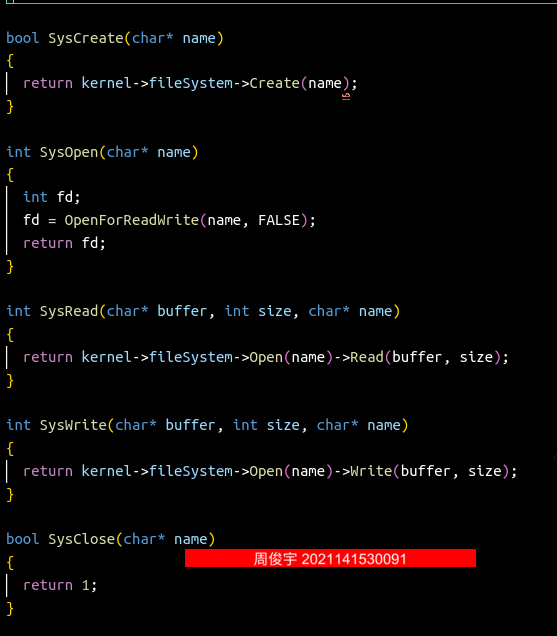
\includegraphics[width=0.6\textwidth]{parts/figures/1.png}
        \end{center}
    }
    \end{minipage}
    \vspace*{2em}

    % \end{minipage}

    }\\\hline
    参考资料和相关网站 & \inlinetable{
        % \nocite{*}
        \bibliography{parts/citation}
    }\\\hline
    本实验的总结 & \inlinetable{
    在 NachOS 文件系统与 shell 实验中,我们学习了文件系统的基本概念和实现方法,以及 shell 的命令行操作和程序执行。通过编写代码和调试,我们深入了解了操作系统的内部工作原理。
        \vspace*{10em}
    }\\\hline
     指导老师评议 & \inlinetable{
         \vspace*{10em}
         \hspace*{2em}成绩评定:\hfill 指导教师签名:\hfill\phantom{0}
     }
	 \\
     \noalign{\hrule height 1pt}
\end{tabularx}